\documentclass[sigconf,anonymous,pbalance]{acmart}
\usepackage{booktabs}
\usepackage{multirow}
\definecolor{hlred}{RGB}{196, 18, 28}
\newcommand{\hl}[1]{\textcolor{hlred}{\mathbf{#1}}}
\newcommand{\hlt}[1]{\textcolor{hlred}{\textbf{#1}}}
\emergencystretch=1.2em

\AtBeginDocument{%
  \providecommand\BibTeX{{%
    Bib\TeX}}}

\setcopyright{cc}
\setcctype{by}
\copyrightyear{2027}
\acmYear{2027}
\acmDOI{10.1145/YYYYYYY.YYYYYYY}

\acmConference[ACMSE 2027]{2027 ACM Southeast Conference}{April 15 to 17, 2027}{Decatur, AL, USA}
\acmBooktitle{2027 ACM Southeast Conference (ACMSE 2027), April 15 to 17, 2027, Decatur, AL, USA}
\acmISBN{979-8-4007-2749-8/2027/04}

\begin{document}
\pagestyle{empty}

\title[Multihorizon Incident Topic Discovery]{Multihorizon Incident Topic Discovery and Shift Tracking Across Enterprise and Open Source Streams}

\author{Anonymous Author}
\affiliation{%
  \institution{Anonymous Institution}
  \city{Anonymous City}
  \state{Anonymous State}
  \country{USA}
}
\email{anonymous@example.edu}

\begin{abstract}
Software reliability teams and enterprise service desks ingest thousands of unstructured bug reports, crash logs, and support requests every quarter, requiring automated methods to group incident descriptions into coherent technical subsystems and detect emerging operational surges. Existing unsupervised topic modeling pipelines struggle on technical ticket streams because bag of words coherence metrics reward models that group recurring ticket boilerplate rather than distinct failure modes, while static two period prevalence comparisons obscure within period volatility and cancel out nonmonotonic monthly waves. We present a multihorizon evaluation framework that pairs dense manifold clustering and domain filtered term weighting with false discovery rate controlled shift testing and continuous trailing rolling window trajectories. Evaluated across open source software engineering issues, enterprise service desk tickets, and a synthetic control benchmark, our framework recovers ground truth operational taxonomies with substantially higher geometric separation and purity than generative and discriminative baselines. Furthermore, it unmasks acute release regressions and monthly provisioning waves that coarse windowing cancels out, while stratifying ticket streams by resolution risk and specialist support queue.
\end{abstract}

\begin{CCSXML}
<ccs2012>
 <concept>
  <concept_id>10010147.10010178.10010179</concept_id>
  <concept_desc>Computing methodologies~Natural language processing</concept_desc>
  <concept_significance>500</concept_significance>
 </concept>
 <concept>
  <concept_id>10010147.10010257.10010258.10010260</concept_id>
  <concept_desc>Computing methodologies~Unsupervised learning</concept_desc>
  <concept_significance>500</concept_significance>
 </concept>
 <concept>
  <concept_id>10011007.10011074.10011111.10011696</concept_id>
  <concept_desc>Software and its engineering~Maintaining software</concept_desc>
  <concept_significance>300</concept_significance>
 </concept>
</ccs2012>
\end{CCSXML}

\ccsdesc[500]{Computing methodologies~Natural language processing}
\ccsdesc[500]{Computing methodologies~Unsupervised learning}
\ccsdesc[300]{Software and its engineering~Maintaining software}

\keywords{Incident Management, Topic Discovery, Density Clustering, Manifold Learning, Temporal Shift Detection, Site Reliability Engineering, Service Desk Triage}

\maketitle

\section{Introduction}
Large scale software systems and enterprise information technology infrastructures generate continuous streams of unstructured diagnostic records, including user submitted bug reports, crash logs, pull requests, and service desk tickets~\cite{agarwal2012identifying, chen2020incidental, he2017drain}. Within both Site Reliability Engineering, which focuses on maintaining the availability and performance of production software services, and Information Technology Service Management, which governs enterprise helpdesk operations and support queues, engineers must continuously triage incoming tickets to distinguish isolated user errors from systemic regressions~\cite{chen2020incidental, vogel2024itsm}. Manual categorization cannot keep pace with rapid release cycles or evolving software dependencies, motivating unsupervised natural language processing methods that group incident descriptions into coherent technical subsystems and track how their prevalence evolves over time~\cite{grootendorst2022bertopic, dieng2020dynamic, zheng2026model}.

\begin{figure*}[t]
  \centering
  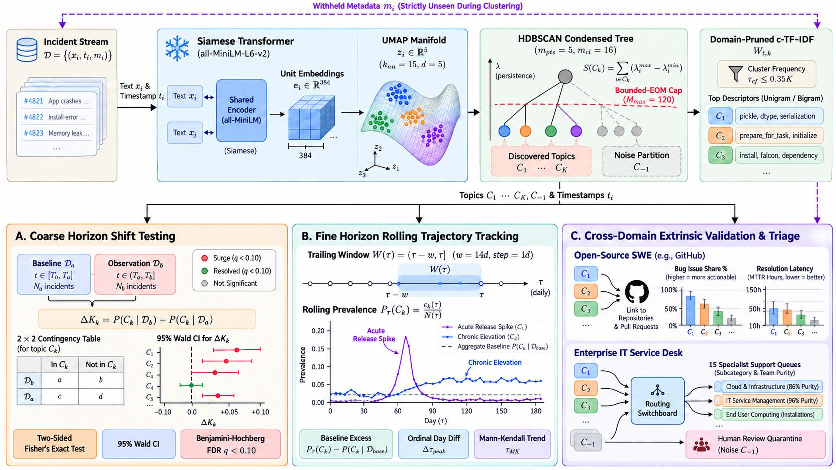
\includegraphics[width=0.92\textwidth]{figures/figure0_pipeline_architecture.pdf}
  \caption{Architecture of the Proposed Multihorizon Incident Topic Discovery and Shift Tracking Pipeline}
  \label{fig:pipeline}
  \Description{Three zone architectural diagram showing (1) Manifold Projection and HDBSCAN Topic Discovery on the left, (2) Multihorizon Shift and Trajectory Analysis in the center, and (3) Cross Domain Extrinsic Validation and Triage on the right.}
\end{figure*}

Despite substantial progress in neural representation learning~\cite{devlin2019bert, reimers2019sentence, wang2020minilm}, unsupervised incident surveillance faces three persistent methodological challenges. First, spatial representation and cluster granularity remain brittle on templated text. Classical probabilistic models such as Latent Dirichlet Allocation (LDA)~\cite{blei2003latent} and Dynamic Embedded Topic Models (DETM)~\cite{dieng2020dynamic} rely on bag of words statistics that are easily distorted by recurring submission headers, while standard word coherence metrics~\cite{newman2010automatic, roder2015exploring} often fail to reflect true subsystem separation~\cite{hoyle2021automated}. Neural clustering pipelines combining pretrained transformers~\cite{reimers2019sentence, sia2020tired} with Uniform Manifold Approximation and Projection (UMAP)~\cite{mcinnes2018umap} and Hierarchical Density Based Spatial Clustering of Applications with Noise (HDBSCAN)~\cite{campello2013density, mcinnes2017hdbscan} overcome lexical sparsity~\cite{grootendorst2022bertopic, bianchi2021pre}, but remain vulnerable to high dimensional distance concentration~\cite{beyer1999nearest} and hierarchical overmerging across related technical vocabularies.

Second, coarse temporal aggregation obscures within period dynamics. Operational studies commonly split a ticket stream into two static eras, such as a baseline window and an observation window, and rank topics by proportional prevalence shift~\cite{chen2020incidental, dieng2020dynamic, grootendorst2022bertopic}. Static two window comparisons harbor two complementary failure modes: when a subsystem experiences a lull followed by a surge within the same window, coarse pooling averages the two phases into false stationarity; conversely, a positive two period delta cannot distinguish an acute release spike that resolved midquarter from a chronic bottleneck that elevated workload throughout the entire period.

Third, single regime evaluation based only on intrinsic metrics limits operational trust. Enterprise helpdesk queues and open source software repositories differ sharply in vocabulary structure, ticket lifecycle, and triage routing~\cite{agarwal2012identifying, vogel2024itsm, lhoest2021datasets}. Judging a model on a single domain or solely by internal word coherence, without testing alignment against ground truth support queues, resolution durations, and bug versus maintenance ratios, offers no guarantee that discovered clusters reflect actionable engineering work~\cite{hoyle2021automated, chen2020incidental}.

We address these challenges through a multihorizon study across an open source software engineering stream~\cite{lhoest2021datasets}, an enterprise service desk corpus~\cite{vogel2024itsm}, and a synthetic control benchmark. Our framework pairs bounded manifold density clustering and domain pruned term weighting with false discovery rate controlled contingency tests~\cite{fisher1922interpretation, benjamini1995controlling}, continuous 14 day rolling trajectories~\cite{mann1945nonparametric, kendall1948rank}, and extrinsic triage validation across domains.

\section{Related Work}
Whereas generative topic models represent documents as mixtures of multinomial word distributions~\cite{blei2003latent, dieng2020dynamic} and mechanistic approaches extract activation directions via sparse autoencoders~\cite{zheng2026model}, short technical tickets dominated by stack traces and version strings favor modular neural pipelines that decouple representation learning from keyword extraction~\cite{sia2020tired, bianchi2021pre, grootendorst2022bertopic}. Following the BERTopic paradigm~\cite{grootendorst2022bertopic}, such pipelines encode documents with pretrained transformers~\cite{reimers2019sentence, wang2020minilm}, reduce dimensionality via UMAP~\cite{mcinnes2018umap}, group dense regions with HDBSCAN~\cite{campello2013density, mcinnes2017hdbscan}, and extract descriptors via class based term weighting. We extend this line of work by analyzing how HDBSCAN cluster selection bounds and domain vocabulary pruning resolve megacluster absorption and expose the failure of sliding window coherence metrics~\cite{newman2010automatic, roder2015exploring, hoyle2021automated} on templated ticket streams.

In software engineering and site reliability operations, automated log parsers such as Drain~\cite{he2017drain} and supervised queue classifiers~\cite{agarwal2012identifying, chen2020incidental} require predefined syntax trees or labeled training histories, limiting their ability to surface novel postrelease failure modes or route unlabeled queues~\cite{chen2020incidental}. Existing unsupervised drift monitors track cluster proportions across discrete time windows~\cite{dieng2020dynamic, grootendorst2022bertopic}, but typically rely on uncalibrated heuristic cutoffs or static window binning that conflate within window volatility with structural shifts. Section~\ref{sec:method} details our spatial and multihorizon temporal framework designed to overcome these limitations.

\section{Methodology}
\label{sec:method}

\subsection{Problem Formulation}
As illustrated in Figure~\ref{fig:pipeline}, our pipeline processes a timestamped stream of technical incident records $\mathcal{D} = \{(x_i, t_i, m_i)\}_{i=1}^{N}$, where $x_i$ combines the ticket title and body text, $t_i$ is the creation timestamp, and $m_i$ denotes operational metadata (resolution timestamps, pull request indicators, or support queues) strictly withheld for extrinsic validation. Fitting the clustering manifold jointly across $\mathcal{D}$ establishes a unified topic taxonomy $\mathcal{C} = \{C_1, \dots, C_K\}$ alongside an explicit noise partition $C_{-1}$, enabling calibrated tests of which subsystems undergo statistically significant prevalence shifts across coarse and fine horizons and how discovered clusters stratify triage outcomes.

\subsection{Manifold Projection and Density Clustering}
Each document $x_i$ is encoded into a unit normalized vector $\mathbf{e}_i \in \mathbb{R}^{D}$ ($D = 384$) using the pretrained \texttt{all-MiniLM-L6-v2} Siamese transformer, which is a dual encoder network trained with a shared weight cosine similarity objective~\cite{reimers2019sentence, wang2020minilm}, and projected onto a low dimensional manifold $\mathbf{z}_i \in \mathbb{R}^{d}$ via UMAP~\cite{mcinnes2018umap} using local neighborhood size $k_{\text{nn}} = 15$ under cosine dissimilarity, zero minimum pack distance, and default dimension $d = 5$. On $\{\mathbf{z}_i\}_{i=1}^{N}$, we apply HDBSCAN~\cite{campello2013density, mcinnes2017hdbscan}. For minimum sample size $m_{\text{pts}} = 5$, the mutual reachability distance between tickets $i$ and $j$ is the maximum of their $m_{\text{pts}}$ nearest neighbor core distances and their Euclidean distance. Constructing a minimum spanning tree yields a hierarchy across density levels $\lambda = 1 / \text{distance}$, where components smaller than minimum cluster size $m_{\text{cl}} = 16$ fall into noise $C_{-1}$ and surviving branches form a condensed tree. Standard HDBSCAN selects flat clusters via Excess of Mass (EOM), maximizing integrated branch persistence:
\begin{equation}
\label{eq:eom}
S(C_k) = \sum_{x_i \in C_k} \left( \lambda_{\text{max}}(x_i, C_k) - \lambda_{\text{min}}(C_k) \right),
\end{equation}
where $\lambda_{\text{min}}(C_k)$ is the density level at which $C_k$ splits from its parent and $\lambda_{\text{max}}(x_i, C_k)$ is the level at which ticket $x_i$ leaves $C_k$. We evaluate both default unbounded EOM and EOM with a maximum cluster size cap of 120 (Bounded EOM, abbreviated BEOM in tables) to prevent parent megaclusters from absorbing distinct subsystems, avoiding the severe outlier rejection of Pure Leaf selection, which extracts only the finest grained terminal leaf nodes at the bottom of the condensed tree.

\subsection{Domain Pruned Class Based Term Weighting}
To extract interpretable topic signatures without generative word priors, we concatenate all documents assigned to cluster $C_k$ and compute class based TF-IDF scores~\cite{grootendorst2022bertopic} over unigrams and bigrams:
\begin{equation}
\label{eq:ctfidf}
W_{t, k} = \frac{f_{t, k}}{\sum_{t' \in \mathcal{V}} f_{t', k}} \cdot \left( \ln \left( \frac{K + 1}{\text{cf}_t + 1} \right) + 1 \right),
\end{equation}
where $f_{t, k}$ is the frequency of term $t$ in $C_k$ and $\text{cf}_t$ is the number of clusters containing $t$. We augment standard English stopwords with a domain boilerplate lexicon and zero out terms whose cluster frequency exceeds $\tau_{\text{cf}} = 0.35 K$, ensuring that top ranked descriptors uniquely characterize the underlying subsystem.

\subsection{Multihorizon Temporal Shift and Trajectory Tracking}
Let $\mathcal{D}_a$ and $\mathcal{D}_b$ denote two nonoverlapping temporal partitions of sizes $N_a$ and $N_b$, where the denominator includes all valid timestamped records, including noise $C_{-1}$, so topic shares reflect true proportions of total operational load. For cluster $C_k$ with ticket counts $c_{k, a}$ and $c_{k, b}$, the coarse prevalence shift is:
\begin{equation}
\label{eq:deltak}
\Delta K_k = P(C_k \mid \mathcal{D}_b) - P(C_k \mid \mathcal{D}_a) = \frac{c_{k, b}}{N_b} - \frac{c_{k, a}}{N_a}.
\end{equation}
We evaluate each $2 \times 2$ contingency table using two sided Fisher's exact tests~\cite{fisher1922interpretation} and construct 95\% Wald confidence intervals, defined as the normal approximation interval for the difference between two independent proportions, for $\Delta K_k$. We then control the familywise false discovery rate (FDR) across all $K$ clusters via the Benjamini and Hochberg step up procedure~\cite{benjamini1995controlling}, which bounds the expected proportion of false positive alerts among all shifts declared significant via adjusted $q$ values.

To resolve within period dynamics, we pair Equation~\ref{eq:deltak} with continuous trailing rolling window tracking. Given a lookback length $w$ in days and a daily step size, each daily endpoint $\tau$ defines a trailing window $\mathcal{W}(\tau) = (\tau - w, \tau]$ containing $N(\tau)$ tickets. Whenever $N(\tau) \ge 5$, we compute the rolling prevalence $P_\tau(C_k) = c_{k}(\tau) / N(\tau)$, retaining tickets from the final $w-1$ days of the preceding quarter so trajectories remain continuous across calendar boundaries. Over any target quarter with $T$ supported daily endpoints, we quantify within quarter evolution through ordinary least squares weekly slopes (in percentage points per week) and the nonparametric Mann and Kendall rank correlation $\tau_{\text{MK}}$~\cite{mann1945nonparametric, kendall1948rank}, which compares concordant and discordant temporal pairs on $[-1, 1]$ to measure monotonic trend consistency. To compare target quarter trajectories against historical behavior, we compute both aggregate baseline relative excess $P_\tau(C_k) - P(C_k \mid \mathcal{D}_{\text{base}})$ and paired ordinal day of quarter differences $P_{j, \text{target}}(C_k) - P_{j, \text{base}}(C_k)$ across comparable days $j \in \{1, \dots, T\}$.

\section{Experimental Setup}

\subsection{Three Regime Benchmark Corpora}
To test whether our framework generalizes across contrasting operational environments, we evaluate the three timestamped corpora summarized in Table~\ref{tab:corpora}. First, the open source software engineering (SWE) stream from the Hugging Face Datasets repository~\cite{lhoest2021datasets} captures rapid release cycles across the first two quarters of 2021. Its withheld metadata distinguishes user reported bug issues from contributor code pull requests (PRs), records maintainer tags, and logs creation and closure timestamps that define Mean Time to Resolution (MTTR), which is the elapsed hours from ticket opening to closure.

\begin{table}[!htbp]
  \caption{Summary of the Three Evaluation Corpora}
  \label{tab:corpora}
  \footnotesize
  \setlength{\tabcolsep}{2.2pt}
  \begin{tabular}{llrrl}
    \toprule
    Regime & Source & $N$ & Horizon & Partitions \& Metadata \\
    \midrule
    Open Source & HF GitHub & 881 & 180d & Q1 (478), Q2 (403); MTTR, PRs \\
    Enterprise IT & Service Desk & 1,380 & 90d+24 & Jan to Mar (1,338), 2024 (42); 15 Teams \\
    Synthetic & Control Sim. & 1,092 & 273d & 3 Quarters; Exact Ground Truth \\
    \bottomrule
  \end{tabular}
\end{table}

Second, the enterprise IT service desk benchmark~\cite{vogel2024itsm} spans a primary first quarter horizon alongside a multiyear follow up slice from 2024. It provides human curated ground truth labels for ticket type (incident versus service request), category, subcategory, priority level, reassignment count, and specialist support queues, plus unassigned Q1 tickets awaiting triage. Third, the synthetic control benchmark embeds three known parametric trajectories (linearly declining, persistent, and linearly emerging) above a constant noise floor across three calendar quarters to verify estimator calibration.

\begin{figure*}[t]
  \centering
  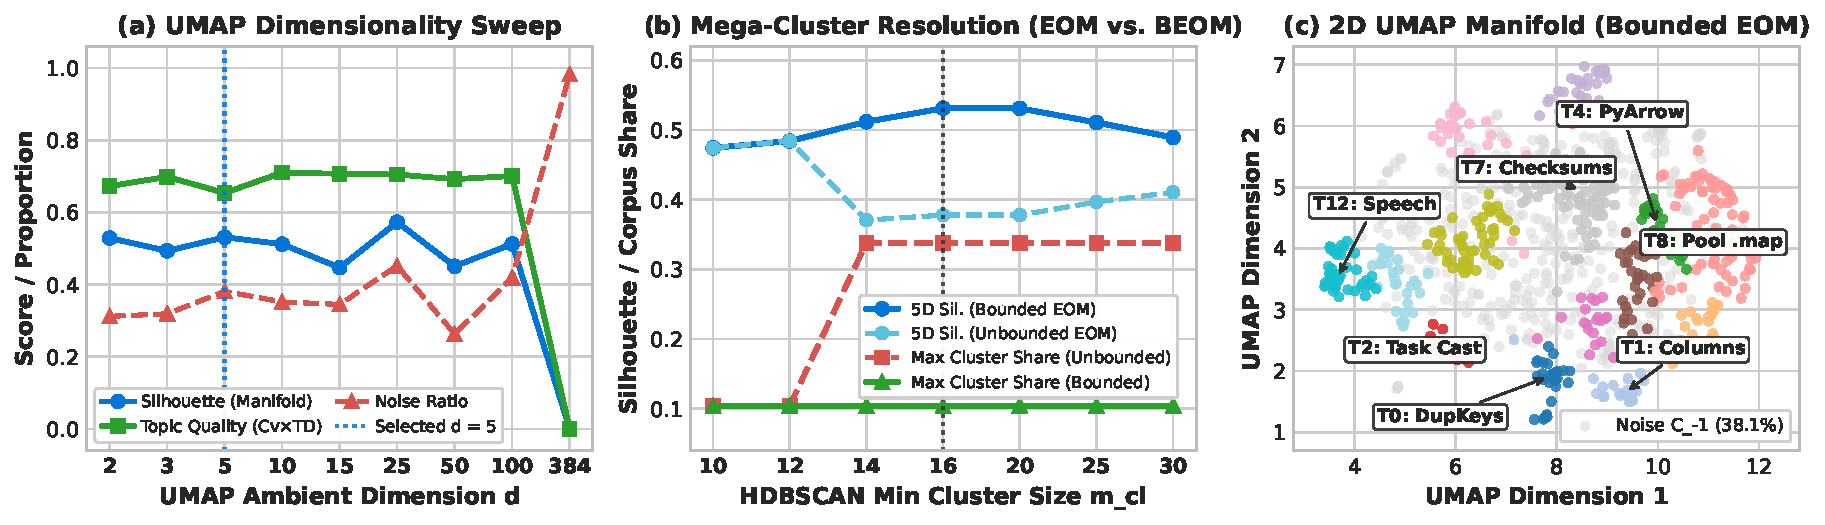
\includegraphics[width=\textwidth]{figures/figure2_spatial_discovery.pdf}
  \caption{Spatial Discovery Analysis: (a) UMAP dimensionality sweep showing a broad stability plateau across $d \in [2, 25]$ before 384D collapse; (b) HDBSCAN megacluster resolution across $m_{\text{cl}} \in [10, 30]$ showing how Bounded EOM cuts largest cluster dominance from 33.8\% to 10.4\% while raising 5D Silhouette; and (c) 2D manifold separation of Bounded EOM subsystems.}
  \label{fig:spatial}
  \Description{Three panel spatial discovery figure showing (a) UMAP ambient dimension sweep from d=2 to d=384, (b) HDBSCAN min_cluster_size sweep comparing Unbounded EOM and Bounded EOM on 5D Silhouette and maximum cluster share, and (c) 2D UMAP manifold scatter plot of Bounded EOM clusters T0 through T12.}
\end{figure*}

\subsection{Baselines and Evaluation Metrics}
We benchmark our pipeline against three baselines across matching cluster counts $K \in \{10, 14, 22\}$ under both standard English and domain pruned stopword filtering: classical generative Latent Dirichlet Allocation (LDA)~\cite{blei2003latent}; sparse discriminative TF-IDF features with $K$-Means (TF-IDF+KM); and dense discriminative $K$-Means applied directly to 384 dimensional Sentence-BERT embeddings (SBERT+KM)~\cite{reimers2019sentence}. Following R{\"o}der, Both, and Hinneburg~\cite{roder2015exploring}, we construct a boolean sliding window index of width 110 tokens and stride 25 tokens to compute Normalized Pointwise Mutual Information (NPMI)~\cite{newman2010automatic}, which normalizes word pair cooccurrence probability by statistical independence. From these scores, we compute $C_v$ coherence by averaging the cosine similarity between each top word's NPMI context vector and the topic's aggregate context vector, Topic Diversity (Div.) as the unique fraction among the top 10 words across all $K$ topics, and Topic Quality as their product ($C_v \times \text{Div.}$). Geometric validity is measured in both the ambient 384D embedding space (Sil.384) and the 5D UMAP manifold (Sil.5D) via the Silhouette coefficient~\cite{rousseeuw1987silhouettes}, which contrasts within cluster cohesion against nearest cluster separation on $[-1, 1]$. Extrinsic alignment against ground truth labels is quantified via Cluster Purity, defined as the fraction of assigned tickets matching their cluster's majority ground truth class.

\section{Spatial Discovery and Granularity Analysis}

\subsection{The Coherence and Geometry Paradox Across Regimes}
Across both operational benchmark corpora, bag of words lexical coherence and geometric cluster validity move in opposite directions in Table~\ref{tab:exp1}. Classical LDA achieves the highest raw $C_v$ coherence under standard stopwords, yet produces negative manifold Silhouette scores on both datasets and ranks last on ground truth support team purity, subcategory purity, and incident versus request purity.

\begin{table}[!htbp]
  \caption{Cross Domain Three Model Benchmark: Domain Pruning Lowers Artificial $C_v$ Inflation While Maximizing Manifold Separation and Ticket Type and Queue Purity}
  \label{tab:exp1}
  \footnotesize
  \setlength{\tabcolsep}{1.8pt}
  \begin{tabular}{llrrrrrr}
    \toprule
    Stream / Filter & Model ($K$) & Noise & $C_v$ & Div. & Sil.384 & Sil.5D & Type / Team \\
    \midrule
    SWE / Std. & LDA (10) & 0.0\% & .948 & .670 & $-.032$ & $-.108$ & None \\
    SWE / Std. & TF-IDF+KM (10) & 0.0\% & .882 & .810 & $-.026$ & $-.168$ & None \\
    SWE / Std. & SBERT+KM (10) & 0.0\% & .853 & .760 & $.026$ & $.043$ & None \\
    SWE / Std. & BEOM (14) & 38.1\% & .862 & .800 & $\hl{.051}$ & $\hl{.531}$ & None \\
    \midrule
    SWE / Pruned & LDA (14) & 0.0\% & .910 & .807 & $-.035$ & $-.225$ & None \\
    SWE / Pruned & TF-IDF+KM (14) & 0.0\% & .718 & 1.00 & $-.034$ & $-.194$ & None \\
    SWE / Pruned & SBERT+KM (14) & 0.0\% & .654 & .943 & $.030$ & $.059$ & None \\
    SWE / Pruned & EOM (10) & 27.2\% & .691 & $\hl{.960}$ & $.026$ & $.378$ & None \\
    SWE / Pruned & BEOM (14) & 38.1\% & .694 & $\hl{.943}$ & $\hl{.051}$ & $\hl{.531}$ & None \\
    \midrule
    IT / Pruned & LDA (14) & 0.0\% & .905 & .836 & $.021$ & $-.060$ & 85.5 / 59.8\% \\
    IT / Pruned & TF-IDF+KM (14) & 0.0\% & .937 & .900 & $.039$ & $.058$ & 92.6 / 72.1\% \\
    IT / Pruned & SBERT+KM (14) & 0.0\% & .874 & .936 & $.083$ & $.269$ & 95.5 / $\hlt{72.3\%}$ \\
    IT / Pruned & EOM (14) & 14.9\% & .840 & $\hl{.979}$ & $\hl{.100}$ & $\hl{.559}$ & 96.6 / 69.2\% \\
    IT / Pruned & BEOM (22) & 34.5\% & .897 & .914 & $\hl{.092}$ & $\hl{.588}$ & $\hlt{98.3}$ / $\hlt{71.3\%}$ \\
    \bottomrule
  \end{tabular}
\end{table}

This divergence stems from how sliding window coherence evaluates cooccurrence in templated technical text~\cite{hoyle2021automated}. In software repositories and enterprise helpdesks, nearly every ticket contains shared scaffolding such as \texttt{dataset}, \texttt{github}, \texttt{https}, \texttt{python}, or \texttt{error message}. Under standard English stopwords, LDA populates multiple topics with slight variations of these ubiquitous template tokens, depressing Topic Diversity in Table~\ref{tab:exp1}. Because template tokens cooccur in almost every sliding window across the corpus, their pairwise NPMI is artificially inflated, driving $C_v$ upward. However, because documents sharing boilerplate words describe unrelated technical subsystems, grouping them together scatters each topic across the semantic embedding space and yields negative Silhouette scores in Table~\ref{tab:exp1}.

Stripping away high frequency boilerplate via domain vocabulary filtering in Table~\ref{tab:exp1} allows class based term weighting to surface specialized subsystem identifiers such as \texttt{duplicated\-keys\-error}, \texttt{prepare\_for\_task}, and \texttt{pyarrow}. Because specialized identifiers occur in narrow, mutually exclusive subsets of tickets, their corpus wide sliding window cooccurrence drops, lowering $C_v$ across all models while substantially raising lexical diversity. Ground truth evaluation on the enterprise stream in Table~\ref{tab:exp1} reveals a key structural distinction between coarse departmental routing and fine grained failure discovery. Whereas forced $K$-Means partitioning (TF-IDF+KM and SBERT+KM) performs competitively on coarse Support Team purity, where every ticket maps into one of 15 broad organizational queues, Bounded EOM leads on both Incident versus Request separation (98.3\%) and fine grained Subcategory purity (82.3\% versus 63.6\% for LDA) alongside the highest manifold Silhouette score (0.588), because density clustering isolates cohesive failure modes while filtering crosscutting noise. Even when noise points are assigned to their nearest centroid to evaluate 100\% of the open source corpus, the UMAP and HDBSCAN pipeline maintains a sixfold advantage in 5D Silhouette over dense $K$-Means ($0.354$ versus $0.059$).

\subsection{Dimensionality Laws and Megacluster Resolution}
Clustering directly in high dimensional transformer space fails without intermediate manifold projection, as shown by the dimensionality sweep~\cite{mcinnes2018umap} in Panel a of Figure~\ref{fig:spatial}. In 384 dimensions, cosine distances between distinct documents concentrate tightly around their mean~\cite{beyer1999nearest}, flattening the mutual reachability graph and erasing the density valleys required to separate clusters so that nearly the entire corpus collapses into noise. Projecting embeddings onto $d \in [2, 25]$ restores steep local density gradients. Crucially, the green Topic Quality curve and blue Manifold Silhouette curve in Panel a of Figure~\ref{fig:spatial} remain jointly flat across the entire $d \in [2, 25]$ range before collapsing together at $d = 384$, demonstrating that manifold density clustering does not depend on fragile dimension tuning once ambient distance concentration is broken.

Within this 5D manifold, comparing the 10 cluster unbounded EOM configuration (R0 through R9) against the 14 cluster Bounded EOM configuration (T0 through T13) across $m_{\text{cl}} \in [10, 30]$ in Panel b of Figure~\ref{fig:spatial} exposes a critical hierarchical overmerging effect on the open source stream~\cite{lhoest2021datasets}. For every $m_{\text{cl}} \ge 14$, unbounded EOM allows a single parent cluster R1 to absorb 33.8\% of the entire corpus, depressing 5D Silhouette to $0.371$--$0.411$. Crosstabulating cluster memberships across the condensed tree reveals that R1 conflates three mechanically distinct subsystems that Bounded EOM separates in Panel c of Figure~\ref{fig:spatial} and Table~\ref{tab:exp2}: multiprocessing worker pool deadlocks in \texttt{.map()} operations (Topic T8), Apache Arrow memory mapped versus disk pointer index collisions in \texttt{load\_from\_disk} (Topic T9), and PyArrow C++ Application Binary Interface (ABI) version mismatches (Topic T4). Because all three subsystems share stack trace tokens such as \texttt{pickle}, \texttt{dtype}, and \texttt{arrow}, their density branches merge at a moderate reachability threshold, causing unconstrained persistence maximization in Equation~\ref{eq:eom}~\cite{campello2013density} to favor their merged ancestor R1 over the individual subsystem branches. Enforcing the Bounded EOM size cap in Panel b of Figure~\ref{fig:spatial} selects the descendant branches instead, holding the largest cluster's corpus share steady at 10.4\% and raising manifold Silhouette above 0.51 across $m_{\text{cl}} \in [14, 25]$. Having established how manifold geometry and bounded tree selection isolate coherent technical subsystems, we next examine how their prevalence evolves across coarse and continuous temporal horizons.

\section{Multihorizon Temporal Shift and Trajectory Analysis}

\subsection{Coarse Quarterly Shifts Versus Rolling Trajectories in Open Source Engineering}
We first validate estimator calibration on the three quarter synthetic control benchmark, where our quarterly contingency tests and rolling estimators recover 100\% of the planted emerging, persistent, and declining trajectories with zero false positive alerts on the stationary noise floor and unbiased linear slope recovery. Applying this calibrated framework to the 14 Bounded EOM subsystems on the open source stream via Fisher's exact tests~\cite{fisher1922interpretation} and Benjamini and Hochberg FDR control~\cite{benjamini1995controlling} in Table~\ref{tab:exp2} yields two substantive insights into repository evolution and statistical power. First, the three statistically significant Q2 surges, namely Multiprocessing Pool Serialization (Topic T8), Task Prompt Casting (Topic T2), and Key Hashing Deduplication (Topic T0), trace back to a single architectural transition in Q2 2021: scaling dataset processing to multiworker parallel execution and standardized task template schemas, which exposed cross process \texttt{pickle} locks and strict shard key uniqueness checks, whereas downloader checksum timeouts (Topic T7) fell following upstream retry patches. Second, comparing Topic T9 against Topics T0 and T2 illustrates why uncalibrated point cutoffs ($|\Delta K| \ge 2.50$ pp) fail: because binomial sampling variance scales with baseline prevalence $p(1-p)$, a $+3.5$ to $+4.1$ pp increase from a near zero Q1 baseline (T0 and T2) represents a $3\times$ to $11\times$ relative outbreak ($q \le 0.028$), whereas a $+2.8$ pp fluctuation atop a large $8.6\%$ baseline in Arrow Disk Indexing (T9) lies well within normal quarterly variance ($q = 0.407$), just like stationary Word Error Rate (WER) metrics (T5), PyArrow ABI (T4), and Automatic Speech Recognition (ASR) audio (T12).

\begin{table}[!htbp]
  \caption{Quarterly Shift Testing on the Open Source Stream: Binomial Baseline Variance Determines Which Surges Survive FDR Control ($q < 0.10$)}
  \label{tab:exp2}
  \footnotesize
  \setlength{\tabcolsep}{2.2pt}
  \begin{tabular}{llrrrrl}
    \toprule
    ID & Technical Subsystem & Q1 & Q2 & $\Delta K$ (95\% CI) & FDR $q$ & Regime \\
    \midrule
    T8 & Pool \texttt{.map()} Pickle & 9.2\% & 15.1\% & $\hl{+5.9}$ ($+1.6, +10.3$) & $\hl{.041}$ & \hlt{Surge} \\
    T2 & Task Prompt Casting & 0.4\% & 4.5\% & $\hl{+4.1}$ ($+2.0, +6.2$) & $\hl{.001}$ & \hlt{Surge} \\
    T0 & DuplicateKeys Hash & 1.7\% & 5.2\% & $\hl{+3.5}$ ($+1.1, +6.0$) & $\hl{.028}$ & \hlt{Surge} \\
    T9 & Arrow Disk Indexing & 8.6\% & 11.4\% & $+2.8$ ($-1.2, +6.8$) & $.407$ & Drift \\
    T5 & WER/BLEURT Metrics & 4.4\% & 5.2\% & $+0.8$ ($-2.0, +3.7$) & $.765$ & Chronic \\
    T4 & PyArrow C++ ABI & 7.1\% & 7.0\% & $-0.2$ ($-3.6, +3.2$) & $1.00$ & Chronic \\
    T12 & Speech ASR Audio & 5.7\% & 3.7\% & $-1.9$ ($-4.7, +0.9$) & $.412$ & Chronic \\
    T7 & Checksum Timeouts & 12.6\% & 7.7\% & $\hl{-4.9}$ ($-8.8, -0.9$) & $\hl{.069}$ & \hlt{Resolved} \\
    \bottomrule
  \end{tabular}
\end{table}

\begin{figure}[!htbp]
  \centering
  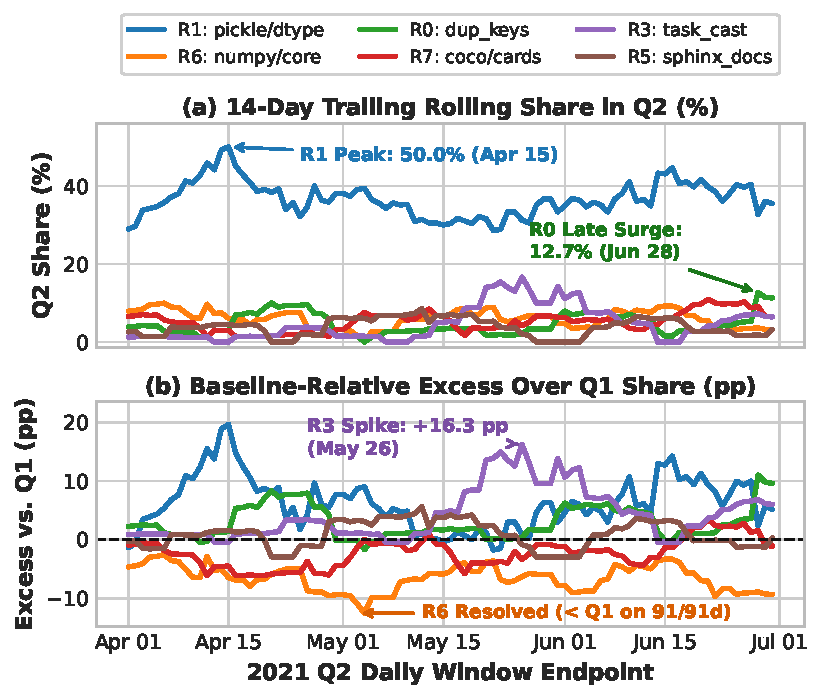
\includegraphics[width=\linewidth]{figures/figure3_q2_rolling_and_excess.pdf}
  \caption{Continuous 14 Day Rolling Trajectories Across Q2 2021: Separating R1's Quarter Long Chronic Elevation From R3's Transient May Feature Sprint}
  \label{fig:q2excess}
  \Description{Two panel time series line chart showing 14 day trailing rolling prevalence across Q2 2021 in the top panel and percentage point excess relative to the Q1 aggregate baseline in the bottom panel.}
\end{figure}

Even when statistically calibrated, coarse two period deltas obscure the within quarter geometry of an outbreak. To maintain dense daily window support ($N(\tau) \ge 5$) across all 91 daily endpoints of Q2 and directly contrast the temporal behavior of the merged parent cluster R1 against individual subsystems, we evaluate 14 day rolling trajectories in the 10 cluster R0 through R9 hierarchy in Table~\ref{tab:q2traj} and Figure~\ref{fig:q2excess}. At the quarterly level, both the merged serialization cluster R1 and the task casting cluster R3 (corresponding to T2) register positive surges, yet their continuous trajectories reflect opposite operational dynamics. Task casting activity in Topic R3 remains dormant through April, erupts into an acute midquarter spike in late May during a coordinated sprint to standardize question answering templates, and subsides in June once those pull requests merge. Conversely, serialization and dtype failures in Topic R1 jump at the start of April and remain chronically elevated above their Q1 norm on nearly every day of Q2. Because R1's step change occurred in early April and plateaued thereafter, its within quarter linear slope and Mann and Kendall trend~\cite{mann1945nonparametric, kendall1948rank} are near zero. An alerting system relying solely on within quarter slopes would miss the largest chronic reliability burden in the repository, whereas one relying solely on quarterly deltas would mistake R3's completed May feature sprint for an active June outage. Meanwhile, duplicate key hashing errors in Topic R0 (T0) accelerate toward a late June peak, Character Error Rate (\texttt{cer\_metric}) evaluation issues in Topic R4 drift modestly upward, and NumPy and checksum errors in Topic R6 (T7) stay below their Q1 norm across every endpoint of Q2.

\begin{table}[!htbp]
  \caption{Second Quarter Rolling Trajectory Diagnostics on the Open Source Stream (Slope in pp/wk; $>$Base = Share of Q2 Windows Above Q1 Baseline)}
  \label{tab:q2traj}
  \footnotesize
  \setlength{\tabcolsep}{1.4pt}
  \begin{tabular}{llrrrrrl}
    \toprule
    ID & Signature & Peak (Date) & Slope & $\tau_{\text{MK}}$ ($p$) & Excess & $>$Base & Regime \\
    \midrule
    R1 & \texttt{pickle/dtype} & \hlt{50.0\% (04/15)} & $-0.06$ & $+0.01$ (.94) & $\hl{+6.29}$ & \hlt{94.5\%} & Chronic \\
    R3 & \texttt{task\_cast} & \hlt{16.7\% (05/26)} & $\hl{+0.52}$ & $\hl{+0.36}$ (\hlt{*1e-6}) & $\hl{+4.26}$ & \hlt{87.9\%} & Spike \\
    R0 & \texttt{dup\_keys} & \hlt{12.7\% (06/28)} & $+0.11$ & $+0.10$ (.15) & $\hl{+2.92}$ & \hlt{87.9\%} & Surge \\
    R5 & \texttt{sphinx\_docs} & 8.6\% (05/12) & $-0.00$ & $+0.00$ (.97) & $+0.90$ & 60.4\% & Routine \\
    R4 & \texttt{cer\_metric} & 9.8\% (06/29) & $+0.03$ & $+0.03$ (.65) & $+0.78$ & 71.4\% & Drift \\
    R2 & \texttt{rename\_col} & 7.3\% (04/27) & $\hl{-0.42}$ & $\hl{-0.58}$ (\hlt{*1e-13}) & $-0.65$ & 46.2\% & Resolved \\
    R9 & \texttt{pdf\_duorc} & 9.2\% (04/01) & $-0.22$ & $\hl{-0.29}$ (\hlt{*5e-5}) & $-1.79$ & 16.5\% & Decline \\
    R7 & \texttt{coco\_cards} & 11.0\% (06/21) & $\hl{+0.34}$ & $\hl{+0.32}$ (\hlt{*8e-6}) & $-2.27$ & 14.3\% & Recovery \\
    R8 & \texttt{speech\_asr} & 8.5\% (05/13) & $-0.20$ & $-0.16$ (.03) & $-3.00$ & 20.9\% & Decline \\
    R6 & \texttt{numpy\_core} & 10.0\% (04/06) & $-0.13$ & $-0.16$ (.03) & $\hl{-6.56}$ & \hlt{0.0\%} & Resolved \\
    \bottomrule
  \end{tabular}
\end{table}

Comparing aggregate baseline excess across 91 endpoints against ordinal day of quarter aligned differences across 77 comparable pairs further underscores the role of baseline selection. While mean excess and mean paired difference agree in sign and magnitude across all topics, pointwise paired differences can be distorted when the baseline quarter experiences a transient local dip on the corresponding ordinal day, as occurs for R1 in mid April because mid January had an unusually low two week ticket volume. Pairing aggregate baseline excess with ordinal alignment prevents analysts from mistaking baseline variance for target quarter anomalies.

\begin{figure*}[t]
  \centering
  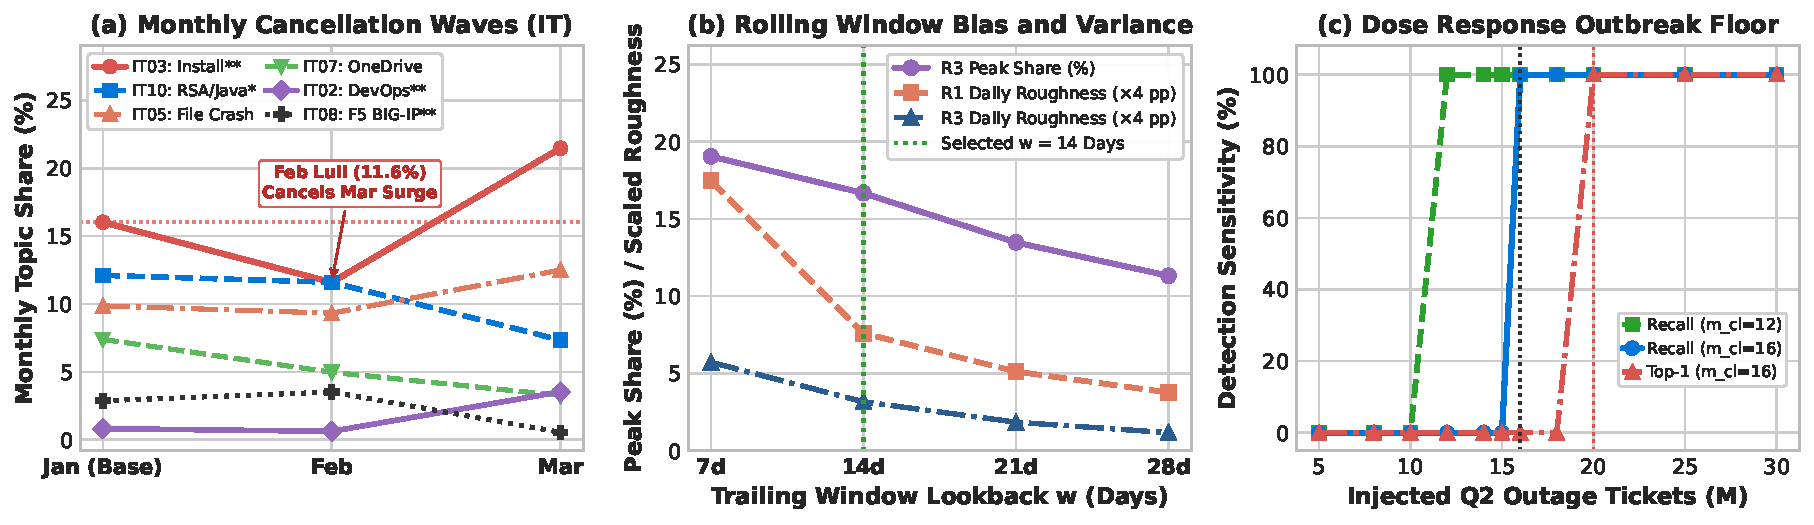
\includegraphics[width=\textwidth]{figures/figure4_temporal_sensitivity.pdf}
  \caption{Multihorizon Sensitivity Laws: (a) Nonmonotonic monthly trajectories on Enterprise IT showing how IT03's February lull cancels its March surge under coarse pooling; (b) rolling lookback bias and variance trade off across $w \in \{7, 14, 21, 28\}$ days (roughness scaled $\times 4$); and (c) step function outbreak detection floor at $M = m_{\text{cl}}$.}
  \label{fig:temporal_sens}
  \Description{Three panel figure showing (a) monthly topic share trajectories across January, February, and March on Enterprise IT illustrating nonmonotonic cancellation in IT03, (b) rolling window lookback sensitivity across w in 7, 14, 21, and 28 days showing peak share versus scaled daily roughness, and (c) dose response outbreak sensitivity floor across injected ticket counts M.}
\end{figure*}

\subsection{How Coarse Windows Mask Regime Shifts in Enterprise IT}
Coarse two period partitioning can make an actively shifting queue appear stationary when subperiod fluctuations move in opposite directions, as shown in Panel a of Figure~\ref{fig:temporal_sens} and Table~\ref{tab:exp8}. Partitioning the Q1 enterprise helpdesk stream~\cite{vogel2024itsm} into January versus pooled February and March yields zero shifts that survive Benjamini and Hochberg FDR control~\cite{benjamini1995controlling}.

\begin{table}[!htbp]
  \caption{Enterprise IT Shift Diagnostics: Fine Horizon Unmasks Four March Shifts That Coarse Pooling Cancels Out (Coarse $\Delta$ Parentheses Show FDR $q$; Peak Is 14d Rolling Max)}
  \label{tab:exp8}
  \footnotesize
  \setlength{\tabcolsep}{1.2pt}
  \begin{tabular}{llrrrrr}
    \toprule
    ID & Subsystem & Peak (Date) & Coarse $\Delta$ & Mar $\Delta$ (95\% CI) & Mar $q$ & $\tau_{\text{MK}}$ \\
    \midrule
    IT03 & Installation & 45.2\% (01/05) & $-0.15$ (.94) & $\hl{+7.65}$ ($+3.0, +12.3$) & $\hl{.007}$ & $\hl{+.17}$ \\
    IT05 & File Crash & 18.4\% (03/11) & $+0.84$ (.90) & $+2.91$ ($-0.9, +6.8$) & $.231$ & $+.26$ \\
    IT02 & DevOps Config & 4.6\% (03/30) & $+1.06$ (.69) & $\hl{+2.81}$ ($+0.9, +4.8$) & $\hl{.007}$ & $\hl{+.46}$ \\
    IT04 & Report Export & 6.0\% (03/13) & $+0.53$ (.88) & $+1.58$ ($-0.2, +3.4$) & $.112$ & $+.28$ \\
    IT01 & Licensing & 22.2\% (01/01) & $-0.31$ (.94) & $+1.40$ ($-2.0, +4.8$) & $.469$ & $+.20$ \\
    IT08 & F5 BIG-IP Err & 5.3\% (01/06) & $-0.64$ (.88) & $\hl{-2.65}$ ($-4.1, -1.2$) & $\hl{.013}$ & $\hl{-.25}$ \\
    IT07 & OneDrive Err & 11.5\% (01/23) & $-3.16$ (.23) & $-2.92$ ($-5.4, -0.4$) & $.112$ & $-.19$ \\
    IT10 & RSA/Java Err & 16.6\% (02/04) & $-2.36$ (.69) & $\hl{-4.52}$ ($-7.9, -1.1$) & $\hl{.059}$ & $\hl{-.27}$ \\
    \bottomrule
  \end{tabular}
\end{table}

The monthly trajectory curves in Panel a of Figure~\ref{fig:temporal_sens} and the statistical tests in Table~\ref{tab:exp8} reveal the mechanism: \textbf{temporal cancellation across nonmonotonic subperiods}. In Cluster IT03, which captures enterprise software installation and upgrade requests, monthly share dips noticeably in February before surging in March during a spring provisioning wave. Pooling February and March averages the February lull with the March surge back to the January baseline, blinding service desk managers to the largest workload wave in the queue. Disaggregating the stream into monthly and 14 day rolling horizons unmasks four statistically significant March regime shifts under Benjamini and Hochberg control: spring rollouts in Software Installations (IT03) and DevOps Custom Configurations (IT02), paired with significant resolutions in F5 BIG-IP Network Errors (IT08) and RSA SecurID and Java Errors (IT10) as winter infrastructure outages were remediated. Furthermore, when the 2024 follow up slice is included, density clustering isolates 100\% of the 2024 records into a dedicated Physical Security and Smart Card Badging cluster, demonstrating that the manifold cleanly separates newly introduced operational categories across multiyear gaps without contaminating historical software queues.

\subsection{Lookback Window Sensitivity and Outbreak Detection Laws}
Selecting the trailing lookback window $w$ and HDBSCAN's minimum cluster size $m_{\text{cl}}$ governs the balance between temporal responsiveness and noise stability, as shown in Panels b and c of Figure~\ref{fig:temporal_sens}. Sweeping $w \in \{7, 14, 21, 28\}$ days in Panel b of Figure~\ref{fig:temporal_sens} exposes a classic bias and variance trade off measured via daily roughness, defined as the mean absolute day to day change $\frac{1}{T-1}\sum_{\tau} |P_\tau(C_k) - P_{\tau-1}(C_k)|$ (scaled $\times 4$ in Panel b for visual comparison against R3's peak share). A 7 day lookback window suffers from severe day to day sample volatility and sparse boundary windows, whereas extending the lookback to 21 or 28 days oversmooths transient outbreaks and delays peak detection by five to eleven days. The sharp knee at $w = 14$ days reflects an operational periodicity: a 14 day trailing window spans exactly two weekly work and sprint cycles, averaging out weekend ticket submission troughs to cut daily roughness by more than half relative to 7 day windows while preserving exact peak timing.

To establish the physical detection floor for emerging outbreaks in the shared manifold, we conduct a controlled dose response perturbation experiment in Panel c of Figure~\ref{fig:temporal_sens} by injecting $M \in [5, 30]$ synthetic outage tickets from three failure families (distributed CUDA and NVIDIA Collective Communications Library (NCCL) out of memory crashes, S3 SSL handshake faults, and Arrow C++ segmentation faults) into Q2. Across all three domains, detection obeys a sharp step function phase transition governed by HDBSCAN's minimum cluster size $m_{\text{cl}}$~\cite{campello2013density}. Below $M < m_{\text{cl}}$, mutual reachability components contain too few vertices to form a valid branch in the condensed tree and fall into noise $C_{-1}$ with zero recall. Exactly at $M = m_{\text{cl}}$, the anomaly condenses into a distinct branch, jumping instantaneously from 0\% to 100\% recall and purity, and becoming the top ranked repository surge once $M$ exceeds the largest natural background shift at 20 tickets. Setting $m_{\text{cl}}$ thus provides reliability engineers with a direct operational guarantee: it specifies the exact minimum ticket volume required to form a distinct topic cluster while ensuring zero false positive clusters below that volume. Beyond statistical detection, however, an operational framework must also demonstrate that discovered clusters map to actionable engineering workflows and triage queues.

\section{Extrinsic Operational Validation Across Regimes}

\subsection{Open Source Engineering: Bug Ratios and Resolution Latency}
If unsupervised text clusters capture genuine engineering subsystems rather than superficial lexical artifacts~\cite{hoyle2021automated}, they should stratify records across withheld operational metrics~\cite{chen2020incidental}. Evaluating the R0 through R9 hierarchy against withheld repository metadata across Figure~\ref{fig:extrinsic_mttr} (user bug share, median turnaround, and unresolved backlog) and Table~\ref{tab:exp6} (PR share, maintainer tags, mean turnaround, and PR filtered shift amplification) shows that discovered clusters partition open source activity into three operational workflow regimes. In Regime I of Figure~\ref{fig:extrinsic_mttr}, documentation builds (Topic R5) and table API refactoring (Topic R2) consist overwhelmingly of contributor PRs rather than user bug reports, resolving rapidly with minimal open backlogs because they represent self contained code submissions verified by continuous integration checks. In Regime II, architectural feature clusters such as Task Casting templates (Topic R3) and PDF/DuoRC dataset parsers (Topic R9) are also PR driven, but require multiweek maintainer design reviews across dataset schemas. In Regime III, clusters capturing C extension compilation and remote checksum failures (Topic R6), shard key hash collisions (Topic R0), and multiprocessing pickle and Arrow dtype crashes (Topic R1) are dominated by user submitted bug issues. Comparing the median turnaround in Figure~\ref{fig:extrinsic_mttr} against the mean MTTR in Table~\ref{tab:exp6} exposes severe right tailed resolution skew in Regime III: in Topic R6, while routine checksum retries resolve within two days at the median, complex macOS and ARM C extension build failures drag the mean resolution time to more than eleven times the median. This workflow separation also explains why filtering out code PRs sharpens incident surge detection in Table~\ref{tab:exp6}: because isolated maintenance PRs disproportionately populate the outlier partition $C_{-1}$, pooling PRs with bug issues dilutes the denominator during reliability outbreaks, whereas evaluating shifts strictly over user reported issues shrinks the outlier share and amplifies the true bug surges in Topics R1 and R0.

\begin{table}[!htbp]
  \caption{Open Source Workflow Diagnostics: Contributor PR Share, Dominant Maintainer Tag, Mean MTTR Tail Latency, and Issue Only Shift Amplification}
  \label{tab:exp6}
  \footnotesize
  \setlength{\tabcolsep}{1.8pt}
  \begin{tabular}{llrlrrrr}
    \toprule
    ID & Signature & PR \% & Dominant Tag & Mean MTTR & All $\Delta$ & Issue $\Delta$ \\
    \midrule
    Noise & Outliers ($C_{-1}$) & \hlt{72.9\%} & \texttt{bug / enh.} & 255.1 h & $-2.19$ & $\hl{-7.21}$ \\
    R1 & \texttt{pickle/dtype} & 48.0\% & \hlt{\texttt{bug (41)}} & 264.4 h & $+7.63$ & $\hl{+11.07}$ \\
    R6 & \texttt{numpy\_core} & 31.3\% & \hlt{\texttt{bug (10)}} & \hlt{422.0 h} & $-6.85$ & $\hl{-11.07}$ \\
    R7 & \texttt{coco\_cards} & 64.3\% & \texttt{dataset req.} & 311.9 h & $-2.57$ & $+0.25$ \\
    R8 & \texttt{speech\_asr} & 65.9\% & \texttt{dataset req.} & 161.8 h & $-2.34$ & $-3.96$ \\
    R5 & \texttt{sphinx\_docs} & \hlt{93.5\%} & \hlt{\texttt{docs (4)}} & \hlt{71.4 h} & $+1.29$ & $+1.24$ \\
    R9 & \texttt{pdf\_duorc} & 64.5\% & \texttt{dataset req.} & 303.2 h & $-2.37$ & $-2.02$ \\
    R0 & \texttt{dup\_keys} & 41.4\% & \hlt{\texttt{bug (6)}} & 157.3 h & $+3.54$ & $\hl{+6.13}$ \\
    R4 & \texttt{cer\_metric} & 48.3\% & \texttt{enh. / bug} & 101.6 h & $+0.79$ & $+1.57$ \\
    R2 & \texttt{rename\_col} & \hlt{80.0\%} & \texttt{enh. / bug} & 269.2 h & $-0.98$ & $+0.27$ \\
    R3 & \texttt{task\_cast} & \hlt{70.0\%} & \hlt{\texttt{enh. (4)}} & 248.1 h & $+4.05$ & $+3.73$ \\
    \bottomrule
  \end{tabular}
\end{table}

\begin{figure}[!htbp]
  \centering
  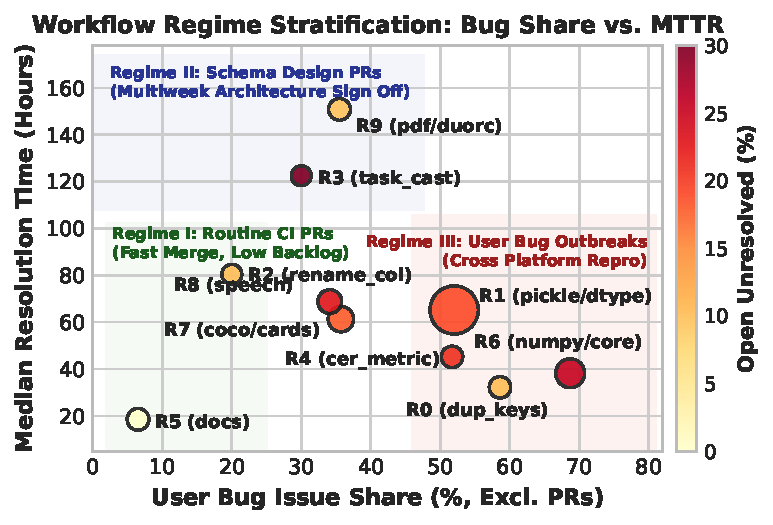
\includegraphics[width=\linewidth]{figures/figure5_extrinsic_mttr.pdf}
  \caption{Workflow Regime Stratification on Open Source Issues: Discovered Topics Separate Into Fast CI PRs (Regime I), Multiweek Schema Reviews (Regime II), and High Backlog User Bug Outbreaks (Regime III)}
  \label{fig:extrinsic_mttr}
  \Description{Scatter plot of user bug issue ratio versus median resolution time in hours across discovered topics R0 through R9 with three shaded operational workflow regimes, sized by ticket volume and colored by open unresolved percentage.}
\end{figure}

\subsection{Enterprise Service Desk: Automated Queue Routing and Service Level Agreement Risk}
On the enterprise service desk corpus~\cite{agarwal2012identifying, vogel2024itsm}, discovered clusters stratify tickets by Service Level Agreement (SLA) risk, which is the operational hazard that resolution exceeds contracted turnaround targets, as shown in Table~\ref{tab:exp9}. Across the queue, resolution latency is governed by \textbf{intake diagnostic ambiguity and Tier 1 escalation bottlenecks}. Routine provisioning clusters such as standard software installations (IT03) or custom DevOps configurations (IT02) map unambiguously at intake to a dedicated fulfillment team such as End User Computing or Software Development and DevOps; because these requests follow deterministic single team runbooks with minimal reassignment, median turnaround remains under four hours with almost no critical escalations. Intermediate application and cloud clusters such as cloud performance degradation (IT09) require localized troubleshooting within Cloud and Infrastructure and average roughly one reassignment hop. At the opposite extreme, Table~\ref{tab:exp9} exposes a striking organizational bottleneck: the five highest latency outage clusters, spanning F5 load balancer faults (IT08), CrowdStrike Falcon endpoint alerts (IT12), RSA token failures (IT10), OneDrive authentication errors (IT07), and Outlook websocket drops (IT06), all share the generic \textbf{IT Service Management} helpdesk as their dominant human assigned queue, suffering median turnarounds of five to ten days and high reassignment counts. Because symptoms of network, endpoint security, and identity outages span multiple infrastructure boundaries, Tier 1 intake agents cannot easily isolate the owning specialist department, leaving tickets to stagnate in the general IT Service Management queue across repeated reassignments. By grouping these contacts directly by their technical failure signature (\texttt{f5 big ip}, \texttt{crowdstrike falcon}, \texttt{ping identity}) and automatically dispatching three quarters of the unassigned Q1 tickets while quarantining ambiguous outliers in $C_{-1}$~\cite{chen2020incidental}, manifold clustering enables intake routing to bypass Tier 1 escalation bottlenecks.

\begin{table}[!htbp]
  \caption{Enterprise Queue Routing and SLA Risk: Cross Boundary Infrastructure Outages Stagnate in Generic IT Service Management Across Multi Hop Reassignments (Inc.\% = Incident Share; Routed = Unassigned Tickets Dispatched; Crit.\% = High/Critical Priority; Med.~m = Median Turnaround in Minutes; Reas. = Mean Reassignments)}
  \label{tab:exp9}
  \footnotesize
  \setlength{\tabcolsep}{2.0pt}
  \begin{tabular}{llrrrrrr}
    \toprule
    ID & Dominant Queue (Purity) & $N$ & Inc.\% & Routed & Crit.\% & Med. m & Reas. \\
    \midrule
    IT00 & IT Service Mgmt (58\%) & 62 & 0\% & 0 & 0.0\% & \hlt{146} & 0.63 \\
    IT01 & Asset \& Vendor (67\%) & 110 & 1\% & 1 & 0.0\% & 222 & \hlt{0.59} \\
    IT02 & SW Dev \& DevOps (\hlt{75\%}) & 20 & 0\% & 0 & 0.0\% & 250 & 0.75 \\
    IT03 & End User Comp. (49\%) & 213 & 14\% & 5 & 5.6\% & \hlt{169} & 0.78 \\
    IT04 & App. Support (\hlt{88\%}) & 21 & 100\% & 5 & 4.8\% & 257 & 1.48 \\
    IT05 & App. Support (63\%) & 139 & 100\% & 15 & \hlt{59.0\%} & 203 & 0.84 \\
    IT09 & Cloud \& Infra (\hlt{86\%}) & 187 & 100\% & $\hl{76}$ & 34.2\% & 417 & 1.22 \\
    IT11 & Security \& Comp. (44\%) & 48 & 100\% & 14 & 37.5\% & 695 & 1.08 \\
    IT13 & Identity \& Access (50\%) & 32 & 100\% & $\hl{30}$ & \hlt{50.0\%} & 7,710 & \hlt{1.59} \\
    IT06 & IT Service Mgmt (50\%) & 26 & 100\% & 8 & 30.8\% & 7,825 & 1.46 \\
    IT08 & IT Service Mgmt (\hlt{83\%}) & 33 & 100\% & $\hl{21}$ & \hlt{57.6\%} & \hlt{8,170} & 1.52 \\
    IT12 & IT Service Mgmt (\hlt{100\%}) & 34 & 100\% & $\hl{25}$ & \hlt{55.9\%} & \hlt{8,272} & \hlt{1.59} \\
    IT10 & IT Service Mgmt (\hlt{94\%}) & 142 & 95\% & $\hl{21}$ & 40.8\% & \hlt{11,944} & 1.42 \\
    IT07 & IT Service Mgmt (\hlt{96\%}) & 72 & 99\% & 16 & 33.3\% & \hlt{15,312} & 1.49 \\
    \bottomrule
  \end{tabular}
\end{table}

\section{Discussion and Conclusion}
Effective incident intelligence requires separating domain boilerplate from subsystem semantics and static period counts from continuous temporal trajectories. Our evaluation across open source software engineering and enterprise service desk streams establishes three operational principles for unsupervised ticket surveillance. First, clustering models should be tuned using low dimensional manifold geometry and bounded HDBSCAN branch selection rather than sliding window word coherence, which rewards recurring ticket templates while masking megacluster collapse. Second, FDR controlled contingency tests must be paired with 14 day rolling trajectories to prevent nonmonotonic monthly cancellation and distinguish transient feature sprints from chronic reliability plateaus, while $m_{\text{cl}}$ defines the exact ticket volume required to trigger a new cluster. Third, building on the shared taxonomy established across historical periods, production deployments can operate inductively between periodic reclusterings by matching incoming tickets against stored cluster centroids while quarantining low similarity residuals in $C_{-1}$ to surface novel failure modes for human review.

\bibliographystyle{ACM-Reference-Format}
\bibliography{references}

\end{document}
